\item O bloco $A$ tem massa de \SI{4}{\kilogram} e o $B$ tem massa de \SI{6}{\kilogram}. Uma mola que tem rigidez $k=\SI{40}{\newton/\meter}$ está
fixada a $B$ e comprimida de \SI{.3}{\meter} contra $A$, como mostra a figura. Determine os ângulos máximos $\theta$ e $\phi$ dos cabos após os blocos serem liberados do repouso e a mola tornar-se não deformada

\begin{center}
	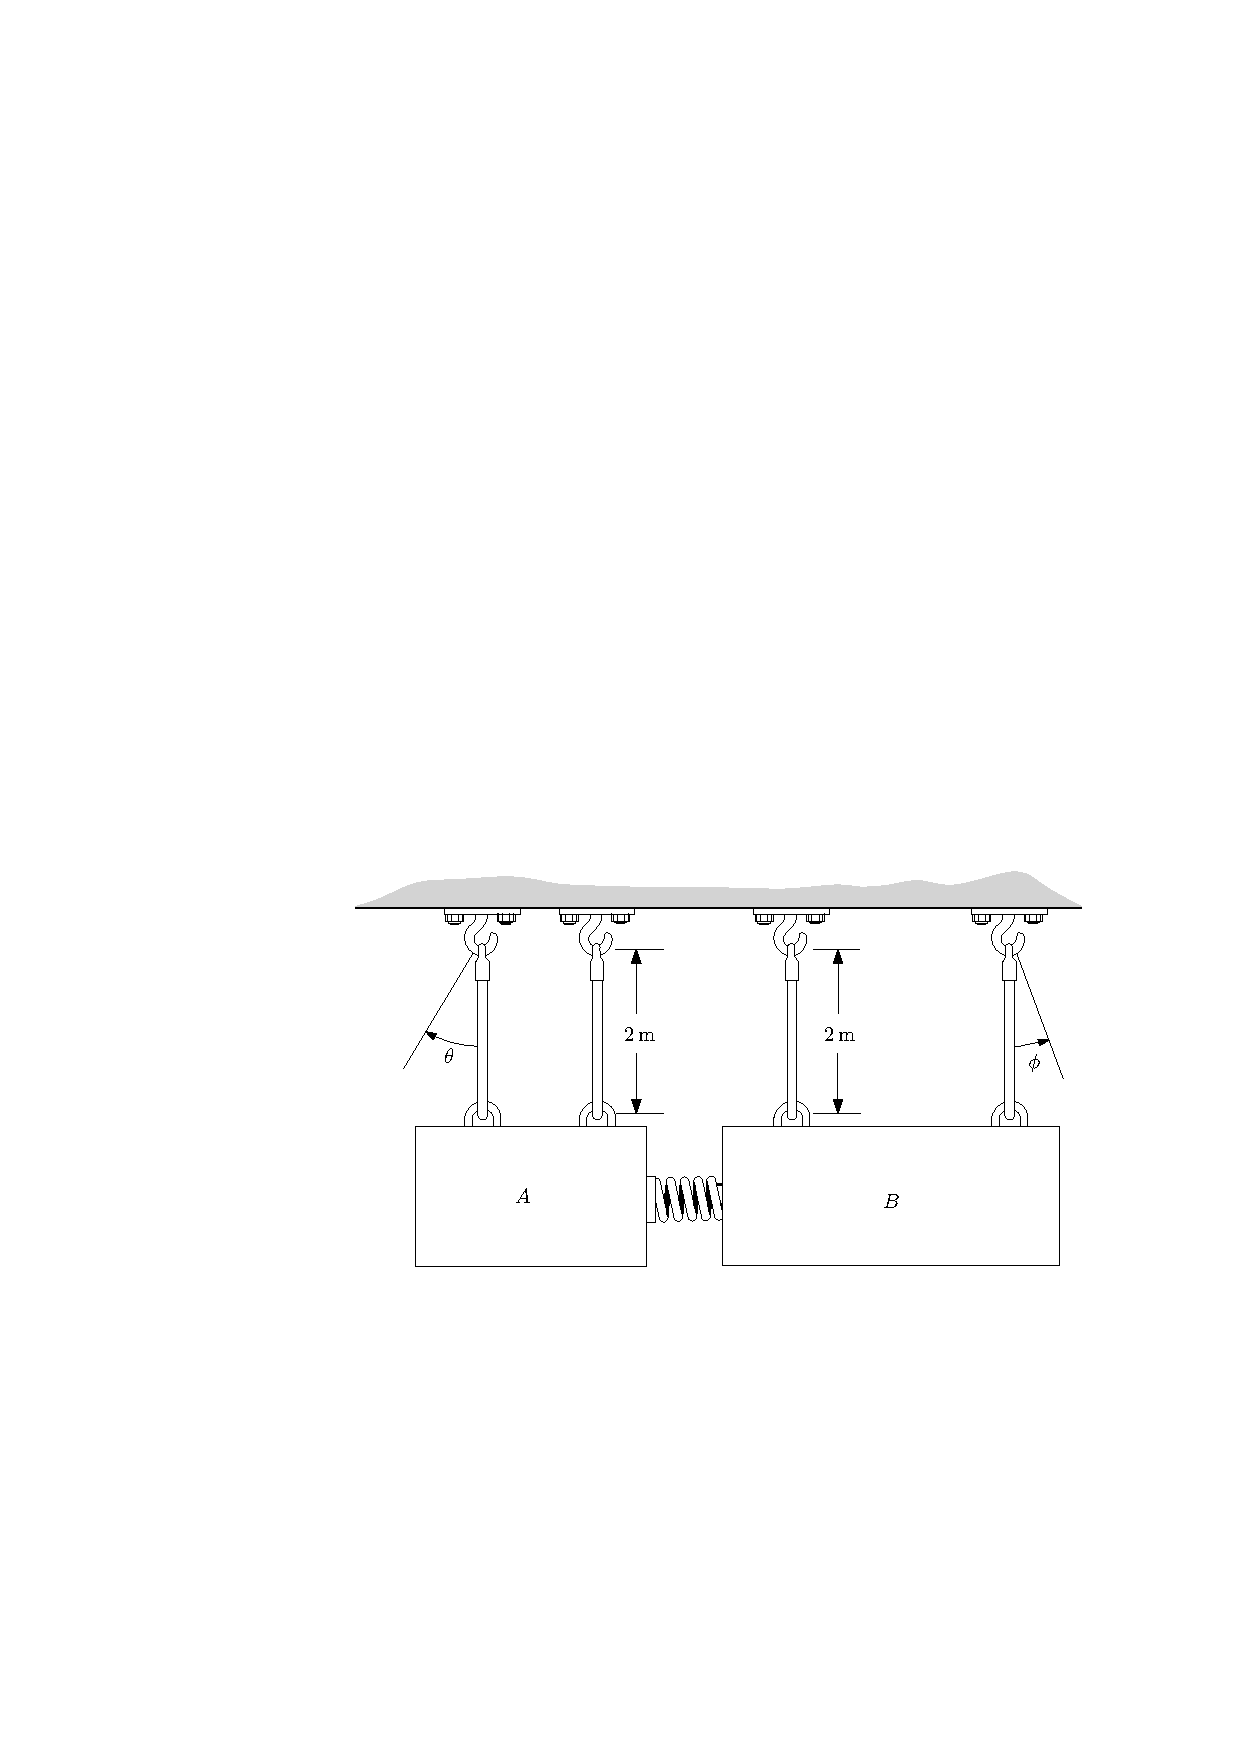
\includegraphics[scale=1.3]{images/draw_2}
\end{center}
